\documentclass{beamer}
% ******************************************************************************
% ****************************** LaTeX Header **********************************
% ******************************************************************************

% ****************************** Custom Margin *********************************
\usepackage{etex}			% An extended version of TEX, controls memory issues.
\usepackage[top=1in, bottom=1in, left=1in, right=1in]{geometry}
\geometry{bindingoffset=0.2in}
\usepackage{enumitem} 		% Control layout of itemize, enumerate, description
\setlength{\parindent}{0 pt}
\setlength{\parskip}{12 pt}

% ******************* Fonts (like different typewriter fonts etc.)*************
\usepackage{amssymb, amsmath, amsthm}
\usepackage{mathtools} 		% Mathematical tools to use with amsmath
\usepackage{dsfont} 		% Doublestroke font
\usepackage{bm} 			% Bold math fonts
%\usepackage{soul} 			 % Hyphenation for letterspacing, underlining, and more

% Palatino for rm and math | Helvetica for ss | Courier for tt
\usepackage{mathpazo} % math & rm
\linespread{1.05}        % Palatino needs more leading (space between lines)
\usepackage[scaled]{helvet} % ss
\usepackage{courier} % tt
\normalfont
\usepackage[T1]{fontenc}

\allowdisplaybreaks


%% test%%
\makeatletter
\def\@makechapterhead#1{%
  %\vspace*{10\p@}%
  {\parindent \z@ 
    {\raggedleft \reset@font
      \fontsize{15ex}{15ex}\selectfont %Problème avec les substitutions...
      \bfseries\thechapter\par\nobreak}%
    \par\nobreak
    \interlinepenalty\@M
    {\raggedright \Huge \bfseries \sffamily #1}%
    \par\nobreak
    \vskip 50\p@
  }}
\def\@makeschapterhead#1{%
  %\vspace*{10\p@}%
  {\parindent \z@ 
    {\raggedleft \reset@font
      \fontsize{15ex}{15ex}\selectfont %Problème avec les substitutions...
      \bfseries\vphantom{\thechapter}\par\nobreak}%
    \par\nobreak
    \interlinepenalty\@M
    {\raggedright \Huge \bfseries \sffamily #1}%
    \par\nobreak
    \vskip 50\p@
  }}

% ************************* Algorithms and Pseudocode **************************
\usepackage{algorithm}
\usepackage{algpseudocode}

% ********************Captions and Hyperreferencing / URL **********************
\usepackage[labelfont=bf,font={small,stretch=0.90},width=0.9\textwidth]{caption}
\usepackage{sidecap} % Typeset captions sideways
\usepackage{subcaption}  % Support for sub-figures and sub-captions
\usepackage{url} % Verbatim with URL-sensitive line breaks
\usepackage[colorlinks=true,linkcolor=black,urlcolor=blue,citecolor=black]{hyperref}

% Fixes a problem with how hyperref records item labels
\makeatletter
\let\oldequation\equation
\renewcommand{\equation}{\@hyper@itemfalse\oldequation}
\let\oldgather\gather
\renewcommand{\gather}{\@hyper@itemfalse\oldgather}
\let\oldalign\align
\renewcommand{\align}{\@hyper@itemfalse\oldalign}
\makeatother

% *************************** Graphics and figures *****************************
\usepackage{rotating}
\usepackage{float}
\usepackage{flafter}	% Ensure floats appear after their definitions.
\usepackage{placeins} 	% For creating float barriers so figure don't span sections
%\restylefloat{figure} % Set figure floating, use \begin{figure}[H] to fix in place.

\usepackage{color}					% color!
\usepackage[x11names]{xcolor}		% ?

% figures, links, etc. 
\usepackage{adjustbox}
\usepackage{graphicx}
\usepackage{pgfplots}
\usetikzlibrary{patterns}	    % in order to define the diagonal hatching
\usetikzlibrary{backgrounds}	% in order to frame a tikzpic
\usetikzlibrary{external} 		% Externalization library to avoid plot re-generation
\tikzexternalize[prefix=Figs/build/] % activate
\pgfplotsset{compat=newest} 
\pgfplotsset{plot coordinates/math parser=false} 
\newlength\figureheight 
\newlength\figurewidth 
\DeclareGraphicsExtensions{.jpg}

% ********************************** Tables ************************************
\usepackage{booktabs}
\usepackage{longtable}
\newcommand{\ra}[1]{\renewcommand{\arraystretch}{#1}}

%\restylefloat{table} % Set table floating, use \begin{table}[H] to fix its position.

\usepackage{multicol}
\usepackage{multirow}
\usepackage{relsize}	% For \mathsmaller command

% ******************************* Line Spacing *********************************
\usepackage{setspace}
\onehalfspacing

% ************************ Formatting / Footnote *******************************
% Don't break enumeration (etc.) across pages in an ugly manner (default 10000)
%\clubpenalty=500
%\widowpenalty=500

%\usepackage[perpage]{footmisc} %Range of footnote options

% *********** To change the name of Table of Contents / LOF and LOT ************
%\renewcommand{\contentsname}{My Table of Contents}
%\renewcommand{\listfigurename}{My List of Figures}
%\renewcommand{\listtablename}{My List of Tables}

% ********************** TOC depth and numbering depth *************************
\setcounter{secnumdepth}{2}
\setcounter{tocdepth}{2}

% ************************* Appendix & Bibliography ****************************
\usepackage{appendix}
\usepackage{natbib}
\usepackage{nomencl}
\makenomenclature
%\renewcommand{\appendixtocname}{List of appendices}
%\renewcommand{\appendixname}{Appndx}

% ******************************** Todo Notes **********************************
\usepackage{fixme}
\renewcommand\fixmelogo{\textsf{TODO:}}
\fxsetup{status=draft}

% ******************************************************************************
% ************************* User Defined Commands ******************************
% ******************************************************************************
% See http://tex.stackexchange.com/questions/1050/whats-the-difference-between-newcommand-and-newcommand for info difference between newcommand and newcommand*

% Changes how \autoref displays the equation reference.
\def\equationautorefname~#1\null{(#1)\null}
%\def\equationautorefname{Equation}
\def\tableautorefname{Table}
\def\figureautorefname{Figure}
\def\subsubsectionautorefname{Subsection}
\def\sectionautorefname{Section}
\def\algorithmautorefname{Algorithm}
% Changes how \eqref displays the equation reference.
%\let\originaleqref\eqref
%\renewcommand{\eqref}{Equation~\originaleqref}
\renewcommand{\eqref}{\autoref}
% Note: autoref makes all of the text link-able, while eqref
% inserts an Eq.~ that cannot be clicked, and a number that can. 
%  i.e., denoting links by [['s, autoref gives something like
%  [[Eq. 1]], while eqref gives something like Eq.~[[(1)]]


% helpful stuff
\newcommand{\code}[1]{{\tt #1}}
\newcommand{\e}[1]{\ensuremath{\times 10^{#1}}}
\newcommand{\ie}{\emph{i.e.,~}}
\newcommand{\eg}{\emph{e.g.,~}}
\newcommand{\etc}{\emph{\textit{etc.}}}
%
\newcommand{\irrats}{\ensuremath{\mathbb{R}\setminus\mathbb{Q}}}
\newcommand{\rats}{\ensuremath{\mathbb{Q}}}
\newcommand{\reals}{\ensuremath{\mathbb{R}}}
\newcommand{\nats}{\ensuremath{\mathbb{N}}}
\newcommand{\ints}{\ensuremath{\mathbb{Z}}}
\newcommand{\complex}{\ensuremath{\mathbb{C}}}
\newcommand{\rp}{\ensuremath{\mathbb{RP}}}
\newcommand{\sph}{\ensuremath{\mathbb{S}}}
%
\newcommand{\abs}[1]{\ensuremath{\left|#1\right|}}
\newcommand{\dee}[2]{\ensuremath{\frac{\mathrm{d}#1}{\mathrm{d}#2}}}
\newcommand{\del}[2]{\ensuremath{\frac{\partial#1}{\partial#2}}}
\newcommand{\csch}{\ensuremath{\mathrm{csch}}}
\newcommand{\caret}{\textasciicircum}
\newcommand{\Siotdac}{Suppose, in order to derive a contradiction~}%
\newcommand{\siotdac}{suppose, in order to derive a contradiction~}%
\newcommand{\Wlog}{Without loss of generality~}%
\newcommand{\ts}{\ensuremath{\textstyle}}
\newcommand{\ds}{\ensuremath{\displaystyle}}
% \wlog is already defined by LaTeX for some reason...
%\newcommand{\wlog}{~without loss of generality~}%
\newcommand{\ld}[2]{\ensuremath{#1_1, \ldots, #1_{#2}}}
\newcommand{\ip}[1]{\ensuremath{\langle #1\rangle}}
% matrix commands 
% (are not working for some reason, so commented out)
% \newcommand{\mat3}[3]{\ensuremath{ \left(
%       \begin{array}{ccc}
%         #1 \\
%         #2 \\
%         #3
%       \end{array}
%       \right)}}

% differential
% \let\oldd\d
\renewcommand{\d}{\ensuremath{\,\mathrm{d}}}

\newcommand\pf{\paragraph{\textbf{\textsc{Proof}}}}
\newcommand\soln{\paragraph{\textbf{\textsc{Solution}}}}
\newcommand\fp{\hfill $\blacksquare$}

% amsthm stuff
\newtheorem{thm}{Theorem}
\newtheorem{prop}[thm]{Proposition}
\newtheorem{coro}[thm]{Corollary}
\newtheorem{lem}[thm]{Lemma}
\newtheorem{defn}[thm]{Definition}
\newtheorem*{ctmcprops}{Properties of a CTMC}

\DeclareMathOperator{\sgn}{\mathrm{sgn}}
\DeclareMathOperator*{\argmax}{arg\,max}
\DeclareMathOperator*{\argmin}{arg\,min}
\DeclareMathOperator{\var}{var}
\DeclareMathOperator{\cor}{cor}
\DeclareMathOperator{\rank}{rank}
\DeclareMathOperator{\countup}{1,2,\ldots}
\DeclareMathOperator{\dist}{d}
\DeclareMathOperator{\intr}{int}
\DeclareMathOperator{\fr}{Fr}
\DeclareMathOperator{\cl}{cl}
\DeclareMathOperator{\Ro}{\mathcal{R}_0}
\DeclareMathOperator{\m}{\mathrm{m}}
\DeclareMathOperator{\pr}{\mathrm{pr}}
\DeclareMathOperator{\torus}{{\mathbb{T}^1}}
\DeclareMathOperator{\Res}{\mathrm{Res}}

\setlist[enumerate, 1]{align=left, label=\arabic*.}
\setlist[enumerate, 2]{align=left, label=(\alph*)}

% [label={\bf \arabic*}.][label=(\roman*)] 

%%%%%%%%%%%%%%%%%%%%%%%%%%%%%%%%%%%%%%%%%%%%%%%%%%%%%%%%%%%%%%%%%%%%%%%
% Macros

% Math Macros.  It would be better to use the AMS LaTeX package,
% including the Bbb fonts, but I'm showing how to get by with the most
% primitive version of LaTeX.  I follow the naming convention to begin
% user-defined macro and variable names with the prefix "my" to make it
% easier to distiguish user-defined macros from LaTeX commands.
%
\newcommand{\myfunction}[3] {${#1} : {#2} \rightarrow {#3}$ }
\renewcommand{\iff}{\Leftrightarrow}
\newcommand{\pluseq}{\mathrel{+}=}
\newcommand{\mineq}{\mathrel{-}=}
\newcommand{\mat}[1]{\boldsymbol{#1}}
\newcommand{\dens}[1]{f_{\uppercase{#1}}(\lowercase{#1})}
\newcommand{\densc}[2]{f_{\uppercase{#1}|\uppercase{#2}}(\lowercase{#1}|\lowercase{#2})}
\renewcommand{\ds}{\,\mathrm{d}s}
\newcommand{\dt}{\,\mathrm{d}t}
\newcommand{\du}{\,\mathrm{d}u}
\newcommand{\dx}{\,\mathrm{d}x}
\newcommand{\dbx}{\,\mathrm{d}\bx}
\newcommand{\dy}{\,\mathrm{d}y}
\newcommand{\dby}{\,\mathrm{d}\by}
\newcommand{\dz}{\,\mathrm{d}z}
\newcommand{\cov}{\mathrm{cov}}

%--------grstep
% For denoting a Gauss' reduction step.
% From the online linear algebra textbook Linear Algebra by Jim Hefferon
% Use as: \grstep{\rho_1+\rho_3} or \grstep[2\rho_5 \\ 3\rho_6]{\rho_1+\rho_3}
\newcommand{\grstep}[2][\relax]{%
   \ensuremath{\mathrel{
       {\mathop{\longrightarrow}\limits^{#2\mathstrut}_{
           \begin{subarray}{l} #1 \end{subarray}}}}}}
    
\newcommand\undermat[2]{%
  \makebox[0pt][l]{$\smash{\underbrace{\phantom{%
    \begin{matrix}#2\end{matrix}}}_{\text{$#1$}}}$}#2}
    
\newcommand\overmat[2]{%
  \makebox[0pt][l]{$\smash{\overbrace{\phantom{%
    \begin{matrix}#2\end{matrix}}}^{\text{$#1$}}}$}#2}
    
% Augmented matrices
\newenvironment{amatrix}[1]{%
  \left[\begin{array}{@{}*{#1}{c}|c@{}}
}{%
  \end{array}\right]
}

% line break within a table cell
% pass [c] or [b] to align with center or bottom of cell
\newcommand{\cellbreak}[3]{%
  \begin{tabular}[#1]{@{}#2@{}}#3\end{tabular}}

\newcommand{\E}{\mathbb{E}}
\newcommand{\R}{\mathbb{R}}
\newcommand{\Z}{\mathbb{Z}}
\newcommand{\F}{\mathbb{F}}
\newcommand{\N}{\mathbb{N}}
\newcommand{\Q}{\mathbb{Q}}
\renewcommand{\P}{\mathbb{P}}

\newcommand{\bS}{\mathbb{S}}
\newcommand{\ba}{\mathbf{a}}
\newcommand{\bb}{\mathbf{b}}
\newcommand{\bc}{\mathbf{c}}
\newcommand{\be}{\mathbf{e}}
\newcommand{\bj}{\mathbf{j}}
\newcommand{\br}{\mathbf{r}}
\newcommand{\bt}{\mathbf{t}}
\newcommand{\bu}{\bm{u}}
\newcommand{\bv}{\mathbf{v}}
\newcommand{\bw}{\mathbf{w}}
\newcommand{\bx}{\bm{x}}
\newcommand{\by}{\bm{y}}
\newcommand{\bz}{\bm{z}}
\newcommand{\bP}{\bm{P}}
\newcommand{\bZ}{\bm{Z}}
\newcommand{\bzero}{\bm{0}}
\newcommand{\bpi}{\bm{\pi}}
\newcommand{\btau}{\bm{\tau}}

\newcommand{\cB}{\mathcal{B}}
\newcommand{\cC}{\mathcal{C}}
\newcommand{\cA}{\mathcal{A}}
\newcommand{\cF}{\mathcal{F}}
\newcommand{\cU}{\mathcal{U}}
\newcommand{\cN}{\mathcal{N}}
\newcommand{\cR}{\mathcal{R}}
\newcommand{\cL}{\mathcal{L}}

\newcommand{\indicator}{\mathds{1}}
\begin{document}
	%\begin{frame}[plain]
\frametitle{Abstract}
\begin{quote}
{\scriptsize
This dissertation demonstrates that there is high revenue potential in using limit order book imbalance as a state variable in an algorithmic trading strategy. Beginning with the hypothesis that imbalance of bid/ask order volumes is an indicator for future price changes, exploratory data analysis suggests that modelling the joint distribution of imbalance and observed price changes as a continuous-time Markov chain presents a monetizable opportunity. The arbitrage problem is then formalized mathematically as a stochastic optimal control problem using limit orders and market orders with the aim of maximizing terminal wealth. The problem is solved in both continuous and discrete time using the dynamic programming principle, which produces both conditions for market order execution, as well as limit order posting depths, as functions of time, inventory, and imbalance. The optimal controls are calibrated and backtested on historical NASDAQ ITCH data, which produces consistent and substantial revenue.}
\end{quote}
\end{frame}

%{
%    \usebackgroundtemplate{
\includegraphics[height=\paperheight,width=\paperwidth]{frames/figs/wordforword.jpg}}
%    \setbeamertemplate{navigation symbols}{}
%    \begin{frame}[plain]
%    \end{frame}
%    }
    \maketitle
    \addtocounter{framenumber}{-2}
    \section*{Roadmap}
    
    {
	\makeatletter \setbeamertemplate{footline}{} \makeatother
    \frame{\frametitle{Roadmap} \tableofcontents}
    }

    \section{Background Information}
    %    % photo of stock market before -- photo of after.
%\begin{frame}
%\frametitle{NYSE Circa 1968}
%\adjustimage{max size=\textwidth}{frames/figs/NYSE_traders_floor.jpg}
%{\tiny This image is available from the United States Library of Congress's Prints and Photographs division under the digital ID ppmsca.03199}
%\end{frame}
%
%\begin{frame}
%\frametitle{NASDAQ Circa Now}
%\adjustimage{max size=\textwidth}{frames/figs/NASDAQ.jpg}
%{\tiny © Copyright 2000, The Nasdaq Stock Market, Inc.
%Reprinted with the permission of The Nasdaq Stock Market, Inc.
%Photo credit: Peter Aaron/Esto }
%\end{frame}
%    
%    % slide on algo/HF trading
%\begin{frame}
%\frametitle{High-Frequency and Algorithmic Trading}
%Hallmarks of HF and Algo trading: algorithms, models, execution speed, timescale. \\
%\vspace{\baselineskip}
%Benefits: 
%\begin{itemize}
%\item reduction of human error 
%\item closes arbitration holes, producing fair markets
%\item digest large sets of data
%\end{itemize}
%\end{frame}
    
    % why do we care? show RenTech profits vs S&P.
\begin{frame}
\frametitle{Why Do We Care?}
\adjustimage{max size=\textwidth}{frames/figs/medallion_returns.jpg}
{\tiny Rubin, R. and Collins, M. (2015). How an exclusive hedge fund turbocharged its retirement plan. \textit{Bloomberg Business.}}
\end{frame}

    % introduce stat arb
    
    % transform ITCH data set into LOB
\begin{frame}[t]
\frametitle{Market Data Feeds}
From the NASDAQ Historical TotalView-ITCH data feed, we receive real-time notification of order arrivals.

\begin{center}
\begin{table}
\begin{tabular}{@{} *{5}{c} @{}}
\toprule
Time & Order ID & Event & Volume & Price \\
\midrule
\vdots & \vdots & \vdots & \vdots & \vdots \\
39960699 &72408630 & 66 & 100 & 1107000 \\
39960710 & 72408630 & 68 & 100 & 1107000 \\
\vdots & \vdots & \vdots & \vdots & \vdots \\
\bottomrule
\end{tabular}
\end{table}
\end{center}
\end{frame}
        
    % introduce LOB
\begin{frame}
\frametitle{Limit-Order Book}
\only<1>{\adjustimage{max size=\textwidth}{frames/figs/LOB1.pdf}}
\only<2>{\adjustimage{max size=\textwidth}{frames/figs/LOB2.pdf}}
\only<3>{\adjustimage{max size=\textwidth}{frames/figs/LOB3.pdf}}
\only<4>{\adjustimage{max size=\textwidth}{frames/figs/LOB4.pdf}}
\end{frame}

    
    \section{Exploratory Data Analysis}
    % introduce CTMC 
\begin{frame}
\frametitle{Limit-Order Book Imbalance}
\emph{Imbalance} is a ratio of quoted limit order volumes between the bid and ask side.
\pause
\[ I(t) = \frac{V_{bid}(t) - V_{ask}(t)}{V_{bid}(t) + V_{ask}(t)} \in [-1,1] \]
\end{frame}

\begin{frame}
\frametitle{Limit-Order Book Imbalance}
\only<1>{\adjustimage{max size=\textwidth}{frames/figs/LOB4.pdf}}
\only<2>{\adjustimage{max size=\textwidth}{frames/figs/LOB4-formula.pdf}}
\end{frame}

\begin{frame}
\frametitle{Limit-Order Book Imbalance}
\only<1>{
Resulting timeseries is noisy.
\adjustimage{max size=\textwidth}{frames/figs/imbalance1.pdf}
}
\only<2>{
Smooth it by averaging on a sliding window (1 s).
\adjustimage{max size=\textwidth}{frames/figs/imbalance2.pdf}
}
\only<3>{
Model as a continuous-time Markov chain $Z(t)$ with generator $G$.
\adjustimage{max size=\textwidth}{frames/figs/imbalance3.pdf}
}
\only<4>{
Model as a continuous-time Markov chain $Z(t)$ with generator $G$.
\vspace{0.1\textwidth}%
\[ \def\arraystretch{2}%
Z = \left\lbrace \begin{array}{lll}
5, & \rho \in [+\frac{3}{5},+1], & \text{buy-heavy} \\
4, & \rho \in [+\frac{1}{5},+\frac{3}{5}], & \text{buy-biased} \\
3, & \rho \in [-\frac{1}{5},+\frac{1}{5}), & \text{neutral} \\
2, & \rho \in [-\frac{3}{5}, -\frac{1}{5}), & \text{sell-biased} \\
1, & \rho \in [-1, -\frac{3}{5}), & \text{sell-heavy} 
\end{array} \right. \]
\vspace{0.1\textwidth}%
}
\end{frame}

% introduce nFPC calibration   
\begin{frame}
\frametitle{Incorporating Price Change}
Next, consider a two-dimensional CTMC $Z(t)$ that jointly models imbalance bin $\rho(t)$ and price change $\Delta S(t)$, where 
\[ \rho(t) \in \lbrace 1,2,\dots,\#_{bins} \rbrace \]
is the bin corresponding to imbalance averaged over the interval $[t-\Delta t_I, t]$, and
\[ \Delta S(t) = \sgn(S(t+\Delta t_S)-S(t)) \in \lbrace -1, 0, 1 \rbrace \]  
is the \emph{sign} of the change in midprice of the \emph{future} time interval $\Delta t_S$.

\adjustimage{max size=\textwidth}{frames/figs/timewindows.pdf}
\end{frame}

% P matrix.
\begin{frame}
\frametitle{Transition Matrix}
Using MLE, we obtain a generator matrix $\mat{G}$ for the CTMC. The transition matrix over a step of size $\Delta t_I$ is given by
\[ \mat{P}(\Delta t_I) = [p_{ij}(\Delta t_I)] = e^{\mat{G} \Delta t_I} \]
called our \emph{one-step transition probability matrix}. Matrix entries give the probability of transition from one (imbalance, price change) pair to another over the time interval $\Delta t_I$. This can be written semantically as
\[ p_{ij} = \mathbb{P}\left[ \varphi( \rho_\text{curr}, \Delta S_\text{future}) = j \; | \; \varphi( \rho_\text{prev}, \Delta S_\text{curr} ) = i \right] \]
\end{frame}

% ... Bayes transform into Q matrix ...
\begin{frame}
\frametitle{Predicting Future Price Change}
Using Bayes' Rule, we can transform the $\mat{P}$ matrix to 
\[ \mathbb{P}\left[ \Delta S_\text{future} = j \; | \; B, \rho_\text{curr} = i \right] = \dfrac{\mathbb{P}\left[ \rho_\text{curr} = i, \Delta S_\text{future} = j \; | \; B \right]}{\mathbb{P}\left[ \rho_\text{curr} = i \; | \; B \right]} \]
This allows us to predict future price moves.
\vspace{\baselineskip}
We'll call the collection of these probabilities the $\mat{Q}$ matrix.
\end{frame}

% show sample Q. 
\begin{frame}
\frametitle{Predicting Future Price Change}
Sample $\mat{Q}$ matrix.
\begin{table}%
\ra{1.2}%
\begin{adjustbox}{width=\textwidth}
\begin{tabular}{@{} r@{\hskip 1cm} *{9}{r} @{}}%
\toprule
& \multicolumn{3}{c}{$\Delta S_\text{curr} < 0$} & \multicolumn{3}{c}{$\Delta S_\text{curr} = 0$} & \multicolumn{3}{c}{$\Delta S_\text{curr} > 0$} \\
\cmidrule(lr){2-4} \cmidrule(lr){5-7} \cmidrule(lr){8-10}
\multicolumn{2}{r}{$\rho_{curr} = 1$} & 2 & 3 & 1 & 2 & 3 & 1 & 2 & 3 \\
\midrule
\multicolumn{10}{l}{$\Delta S_\text{future} < 0$} \\
$\hphantom{abcd}\rho_\text{prev} = 1$ & \bf 0.53 & 0.15 & 0.12 & 0.05 & 0.10 & 0.14 & 0.08 & 0.13 & 0.14 \\
$\rho_\text{prev} = 2$ & 0.10 & \bf 0.58 & 0.14 & 0.07 & 0.04 & 0.10 & 0.13 & 0.06 & 0.12 \\
$\rho_\text{prev} = 3$ & 0.08 & 0.12 & \bf 0.52 & 0.09 & 0.06 & 0.03 & 0.11 & 0.10 & 0.05 \\[0.6ex]
\multicolumn{10}{l}{$\Delta S_\text{future} = 0$} \\
$\rho_\text{prev} = 1$ & 0.41 & 0.75 & 0.78 & \bf 0.91 & 0.84 & 0.79 & 0.42 & 0.79 & 0.77 \\
$\rho_\text{prev} = 2$ & 0.79 & 0.36 & 0.71 & 0.83 & \bf 0.92 & 0.82 & 0.75 & 0.37 & 0.78 \\
$\rho_\text{prev} = 3$ & 0.79 & 0.74 & 0.40 & 0.81 & 0.83 & \bf 0.91 & 0.70 & 0.76 & 0.39 \\[0.6ex]
\multicolumn{10}{l}{$\Delta S_\text{future} > 0$} \\
$\rho_\text{prev} = 1$ & 0.06 & 0.10 & 0.09 & 0.04 & 0.06 & 0.07 & \bf 0.50 & 0.09 & 0.09 \\
$\rho_\text{prev} = 2$ & 0.10 & 0.06 & 0.15 & 0.10 & 0.04 & 0.08 & 0.12 & \bf 0.57 & 0.10 \\
$\rho_\text{prev} = 3$ & 0.13 & 0.14 & 0.08 & 0.10 & 0.11 & 0.05 & 0.19 & 0.14 & \bf 0.56 \\
\bottomrule
\end{tabular}%
\end{adjustbox}%
\end{table}%
\end{frame}

% present Naive strategies 1-3
\begin{frame}
\frametitle{Trading Strategies Informed by the $\mat{Q}$ Matrix}
\begin{itemize}
\item[Naive] Use market orders to buy (sell) if price is predicted to move up (down).
\item[Naive+] Post at-the-touch limit orders when zero price change is predicted.
\item[Naive++] Post a limit order to buy (sell) is price is predicted to move up (down).
\end{itemize}
\end{frame}

\begin{frame}
\frametitle{Calibration of Naive Trading Strategies}
Need to select:
\begin{itemize}
\item price change observation period $\Delta t_S$
\item imbalance averaging period $\Delta t_I$
\item number of imbalance bins $\#_{bins}$
\end{itemize}
Calibration done on the first day of the trading year, same parameters used for all days.

Brute-force search of parameter space, using max Sharpe ratio criterion, found that $\Delta t_S = \Delta t_I = 1 sec$, and $\#_{bins} = 4$
\end{frame}

% present plots
\begin{frame}
\frametitle{Results of Naive Trading Strategies}
\begin{figure}%
\centering%
\subfloat{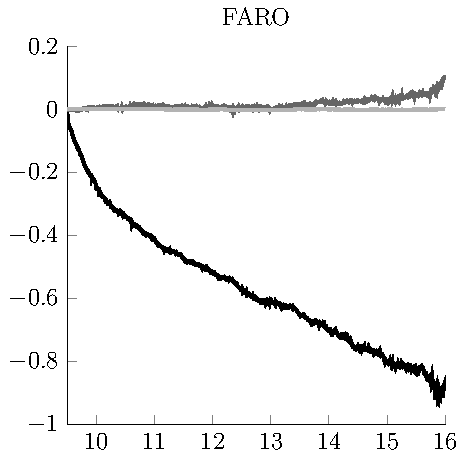
\includegraphics[height=.3\textwidth, width=.35\textwidth]{frames/figs/FARO_naive_strat_comp.pdf}}\quad
\subfloat{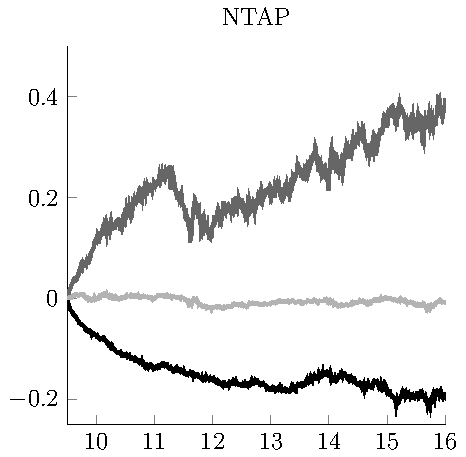
\includegraphics[height=.3\textwidth, width=.35\textwidth]{frames/figs/NTAP_naive_strat_comp.pdf}}\\
\subfloat{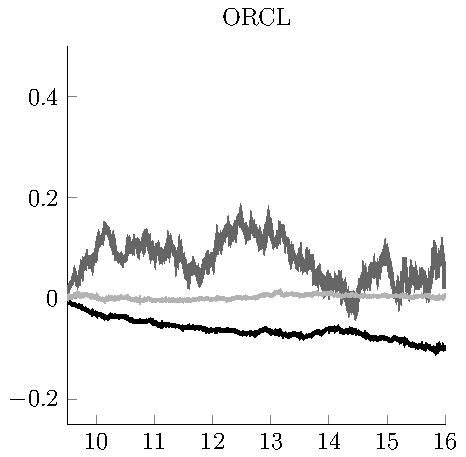
\includegraphics[height=.3\textwidth, width=.35\textwidth]{frames/figs/ORCL_naive_strat_comp.pdf}}\quad
\subfloat{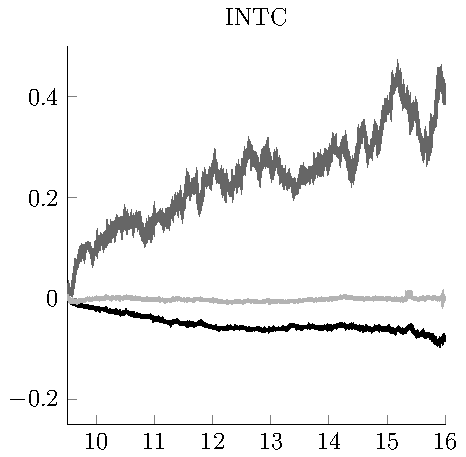
\includegraphics[height=.3\textwidth, width=.35\textwidth]{frames/figs/INTC_naive_strat_comp.pdf}}\\
%
\leavevmode\smash{\makebox[0pt]{\hspace{2em}% HORIZONTAL POSITION           
  \rotatebox[origin=l]{90}{\hspace{3em}% VERTICAL POSITION
	Normalized Profit and Loss (P\&L)}%
}}\hspace{0pt plus 1filll}\null%

Time (h)

\vspace{1cm}%
\subfloat{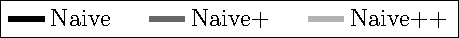
\includegraphics[scale=1]{frames/figs/naivestratlegend.pdf}}%
\end{figure}

\end{frame}

% talk about calibration and failures
\begin{frame}
\frametitle{Conclusions from Naive Trading Strategies}
{\bf Why is the Naive strategy producing, on average, normalized losses?}
\begin{itemize}
\item Backtest is out-of-sample; evidence to reject time-homogeneity
\item Calibration is done on first trading day; likely nonrepresentative of trading activity
\item Price change probability matrix $\mat{Q}$ obtained using midprices, ignoring bid-ask spread; $\sgn(\Delta S)$ may be insufficient for create profit, especially on \texttt{FARO}
\end{itemize}
\end{frame}

\begin{frame}
\frametitle{Conclusions from Naive Trading Strategies}
{\bf Why do the Naive+ and Naive++ strategies outperform the Naive strategy?}
\begin{itemize}
\item LOs vs MOs means different transaction price is being used (only MO loses value)
\item Naive only executes when predicting non-zero price change
\begin{itemize}
\item Only sign, not magnitude
\item Only \emph{if one was already seen}
\end{itemize}
\end{itemize}
\end{frame}

    
    %\section{Maximizing Wealth via Continuous-Time Stochastic Control}
    %% system description - each variable.
\begin{frame}
\frametitle{System Description}
\begin{itemize}
\item Imbalance Averaging Time $\Delta {t_{I}}$ \\
    A constant, specifying the time window over which the imbalance ratio $I(t)$ will be averaged.
\item Price Change Time $\Delta {t_{S}}$ \\
    A constant, specifying the time window over which price changes will be computed.
\item Number of Imbalance Bins $\#_{bins}$ \\ 
    A constant, specifying the number of bins (spaced by percentiles, symmetric around zero) into which $I(t)$ will be sorted.
\item Imbalance $\rho_t$ \\
    The finite, discrete stochastic process that results from sorting $I(t)$ into the imbalance bins $\{1, \dots, \#_{bins} \}$, and which evolves in accordance with the CTMC $\bZ$.
\end{itemize}
\end{frame}

\begin{frame}
\frametitle{System Description}
\begin{itemize}
\item Midprice $S_t$ \\
    Stochastic process, evolves according to CTMC $\bZ$.
\item Midprice Change $\Delta S_t = \sgn(S_t - S_{t-\Delta {t_{S}}})$
\item Imbalance \& Midprice Change $\bZ_t = (\rho_t, \Delta S_t) $ \\
    Continuous-time Markov chain with generator $\mat{G}$.
\item Bid-Ask Half-Spread $\xi$ \\
    Assumed constant. $2\xi$ is equal to the bid-ask spread.
\item Midprice Change $\{ \eta_{0,\bz}, \eta_{1,\bz}, \dots \} \sim F_{\bz}$ \\
    i.i.d. RVs, with distribution dependent on the Markov chain state.
\end{itemize}
\end{frame}

\begin{frame}
\frametitle{System Description}
\begin{itemize}
\item Other Agent Market Orders $K^{\pm}_t$ \\
    Poisson processes with rate $\mu^{\pm}(\bZ_t)$. $K^+$ represents the arrival of another agent's buy market order.
\item Our Limit Order Posting Depth $\delta^{\pm}_t$ \\
    One of our controlled $\cF$-predictable processes. $\delta^+$ dictates how deep on the buy side we will post our buy limit order; $\delta^+ = 0$ implies at-the-touch.
\item Our Limit Order Fill Count $L^{\pm}_t$ \\
    Counting processes (not Poisson), satisfying
    \[ \P [\d L^{\pm}_t = 1 \, | \, \d K^{\mp}_t = 1] = e^{-\kappa \delta^{\pm}_t} \]
\end{itemize}
\end{frame}

\begin{frame}
\frametitle{System Description}
\begin{itemize}
\item Fill Probability Constant $\kappa$ \\
    Fitted to satisfy the above relation, by considering the avg vol available at the first few depths relative to distribution of volumes of incoming market orders
\item Our Market Orders $M^{\pm}_t$ \\
    $M^+$ represents our buy market order. Assume we achieve the best bid/ask price.
\item Our Market Order Execution Times $\btau^\pm = \{ \tau^\pm_k : k = 1, \dots \}$ \\
    An increasing sequence of $\cF$-stopping times.
\end{itemize}
\end{frame}

\begin{frame}
\frametitle{System Description}
\begin{itemize}
\item Cash $X^{\btau, \delta}_t$ \\
    A stochastic variable representing our cash, initially zero, that evolves according to
\[ \begin{aligned}
\d X^{\btau, \delta}_t = & \underbrace{(S_t + \xi + \delta^{-}_t) \d L^{-}_t}_{\text{sell limit order}} - \underbrace{(S_t - \xi - \delta^{+}_t) \d L^{+}_t}_{\text{buy limit order}} \\
                         & + \underbrace{(S_t - \xi) \d M^{-}_t}_{\text{sell market order}} - \underbrace{(S_t + \xi) \d M^{+}_t}_{\text{buy market order}}
\end{aligned} \]
\item Inventory $Q^{\btau, \delta}_t$ \\
    A stochastic process representing our assets, initially zero, that satisfies
\[ Q^{\btau, \delta}_0 = 0, \qquad Q^{\btau, \delta}_t = L^+_t + M^+_t - L^-_t - M^-_t \]
\end{itemize}
\end{frame}

\begin{frame}
\frametitle{Terminal Wealth}
Call $W^{\btau, \delta}_t$ our net present value (NPV) at time $t$.
Hence $W^{\btau, \delta}_T$ at terminal time $T$ is our `terminal wealth.' 

At $T$, we:
\begin{itemize}
\item finish each trading day with zero inventory (avoid overnight positional risk)
\item submit a market order (of a possibly large volume) to liquidate remaining stock
\item price achieved will be $S - \xi \sgn Q - \alpha Q$
\begin{itemize}
\item $\xi \sgn Q$ represents crossing the spread
\item $\alpha$ is a penalty constant
\item $\alpha Q$ represents receiving a worse price linearly in $Q$ due to walking the book
\end{itemize}
\end{itemize}

Hence, $W^{\btau, \delta}_t$ satisfies:
\[
W^{\btau, \delta}_t = \underbrace{\vphantom{\left( Q^{\btau, \delta}_t) \right)}X^{\btau, \delta}_t}_{\text{cash}}+ \underbrace{Q^{\btau, \delta}_t \left( S_t - \xi \sgn(Q^{\btau, \delta}_t) \right)}_{\text{book value of assets}} - \underbrace{\alpha \left( Q^{\btau, \delta}_t \right)^2}_{\text{liquidation penalty}}
\]
\end{frame}

% perf crit and value func
\begin{frame}
\frametitle{Dynamic Programming Value Function}
Our performance criterion will be to maximize terminal wealth:
\[
H^{\btau, \delta}(t,x,s,\bz,q) = \E_{t,x,s,z,q} \left[ W_T^{\btau, \delta} \right]\vphantom{\int\limits_t^T}
\]

The \emph{value function} is given by
\[
H(t,x,s,\bz,q) = \sup\limits_{\btau \in \mathcal{T}_{[t,T]}} \sup\limits_{\delta \in \cA_{[t,T]}} H^{\btau, \delta}(t,x,s,\bz,q)
\]

Admissible trading strategies is the product of the set $\mathcal{T}$ of all $\cF$-stopping times, with the set $\cA$ of all $\cF$-predictable, bounded-from-below depths $\delta \geq 0$.
\begin{itemize}
\item recognizing $\tau$ does not require knowledge of the future
\item $\delta$ cannot `see into the future'; measurable with respect to information at an earlier time
\end{itemize}
\end{frame}

% solve dH...
\begin{frame}
\frametitle{Dynamic Programming Equation}
\begin{theorem}{\bf Dynamic Programming Equation for Optimal Stopping and Control.} \textit{(Cartea et al., 2015)} Assume that the value function $H(t,\bx)$ is once differentiable in $t$, all second-order derivatives in $\bx$ exist, and that $G : \R^m \rightarrow \R$ is continuous. Then $H$ solves the quasi-variational inequality
\[
\max \left\lbrace \partial_t H + \sup \limits_{\bu \in \cA_t} \cL^{\bu}_t H \; ; \; G - H \right\rbrace = 0
\]
on $\mathcal{D}$, where $\mathcal{D} = [0,T] \times \R^m$.
\end{theorem}
\end{frame}

\begin{frame}
\frametitle{Solving for the Infinitesimal Generator}
\[
\begin{aligned}
& \d H (t,x,s,\bz,q) = \partial_t H \d t \\
& \hphantom{\partial_t H} + \underbrace{e^{ -\kappa \delta^{-}} \bigl[ H(t,x+(s+\xi+\delta^-),s,\bz,q-1) - H(\cdot) \bigr] \d K^+}_{\text{probability of our sell limit order being filled, times the change in value}} \\
& \hphantom{\partial_t H} + \underbrace{e^{ -\kappa \delta^{+}} \bigl[ H(t,x-(s-\xi-\delta^+),s,\bz,q+1) - H(\cdot) \bigr] \d K^-}_{\text{probability of our buy limit order being filled, times the change in value}} \\
& \hphantom{\partial_t H} + \sum_{\bj} \underbrace{\E \left[ H(t,x,s+\eta_{0,\bj},\bj,q) - H(\cdot) \right] \d Z_{\bz,\bj}}_{\text{change in value resulting from a CTMC state switch}}
\end{aligned}
\]
\end{frame}

% comp proc for Markov chain
\begin{frame}
\frametitle{Compensated Markov Chain Process}
To solve for $\cL^{\bu}_t Ht$ we need the compensated Markov chain process.
For Poisson processes, this is
\[ \d K^{\pm} = \d \simcal{K}^{\pm} + \mu^{\pm}(\bz) \d t \]
%\vspace{\baselineskip}
For the CTMC:
\begin{itemize}
\item Define $K_l(t)$ to be the number of jumps with $Z_s - Z_{s^-} = l$ up to time $t$ 
\item Define $\beta_l(x) = G_{x,x+l}$
\item Then the compensated process (a martingale) is \[ \simcal{K}_l(t) = K_l(t) - \int_0^t \beta_l(Z_s) \d s \]
\end{itemize}
\end{frame}

% inf gen
\begin{frame}
\frametitle{Solving for the Infinitesimal Generator}
\[
\resizebox{\textwidth}{!}{$\displaystyle
\begin{aligned}
\cL^{\delta}_t H & = \mu^+(\bz) e^{ -\kappa \delta^{-}} \bigl[ H(t,x+(s+\xi+\delta^-),s,\bz,q-1) - H(\cdot) \bigr] \\
& \quad + \mu^-(\bz) e^{ -\kappa \delta^{+}} \bigl[ H(t,x-(s-\xi-\delta^+),s,\bz,q+1) - H(\cdot) \bigr] \\
& \quad + \sum_{\bj} G_{\bz,\bj} \E \left[ H(t,x,s+\eta_{0,\bj},\bj,q) - H(\cdot) \right]
\end{aligned}
$}
\]
\end{frame}

% resulting DPE w/ bdry cond
\begin{frame}
\frametitle{Resulting Dynamic Programming Equation}
Our dynamic programming equation simplifies to
\[
\resizebox{\textwidth}{!}{$\displaystyle
\begin{aligned}
0 = \max \biggl\lbrace \partial_t H + \sup \limits_{\bu \in \cA_t} \cL^{\bu}_t H \; ; \; & H(t,x-(s+\xi), s, \bz, q+1) - H(\cdot) \; ; \\
&  H(t,x+(s-\xi), s, \bz, q-1) - H(\cdot) \biggr\rbrace
\end{aligned}
$}
\]
with boundary conditions
\begin{align*}
H(T, x, s, \bz, q) & = x + q(s - \xi \sgn (q)) - \alpha q^2 \\
H(t, x, s, \bz, 0) & = x
\end{align*}
\end{frame}

% ansatz
\begin{frame}
\frametitle{Ansatz for Value Function $H$}
Introduce the ansatz 
 \[ H(t, x, s, \bz, q) = x + q(s - \xi \sgn(q)) + h(t,\bz,q) \]
\begin{itemize}
\item separates out mark-to-market of the current position
\item $h(t,\bz,q)$ captures value due to optimal trading
\end{itemize}
Boundary conditions on $h$ are
\begin{align*}
h(T, \bz, q) & = - \alpha q^2 \\
h(t, \bz, 0) & = 0
\end{align*}
\end{frame}

% simplified inf gen with sgn
\begin{frame}
\frametitle{Simplified Infinitesimal Generator}
\[
\resizebox{\textwidth}{!}{$\displaystyle
\begin{aligned}
\cL^{\delta}_t H & = \mu^+(\bz) e^{ -\kappa \delta^{-}} \bigl[ \delta^- + 2 \xi \cdot \indicator_{q \geq 1} + h(t,\bz,q-1) - h(t,\bz,q) \bigr] \\
& \quad + \mu^-(\bz) e^{ -\kappa \delta^{+}} \bigl[ \delta^+ + 2 \xi \cdot \indicator_{q \leq -1} + h(t,\bz,q+1) - h(t,\bz,q) \bigr] \\
& \quad + \sum_{\bj} G_{\bz,\bj} \left[q \E [\eta_{0,\bj}] +h(t,\bj,q) - h(t,\bz, q) \right]
\end{aligned}
$}
\]
\end{frame}

% opt posting d+ and floored d+
\begin{frame}
\frametitle{Optimal Posting Depth}
To find the supremum over $\delta^+$, consider the first-order constraint:
\[
\resizebox{\textwidth}{!}{$\displaystyle
\begin{aligned}
0 & = \partial_{\delta^+} \biggl[ e^{ -\kappa {\delta^+}^*} \bigl[ {\delta^+}^* +  2 \xi \cdot \indicator_{q \leq -1} + h(t,\bz,q+1) - h(t,\bz,q) \bigr] \biggr] \\
& = -\kappa e^{ -\kappa {\delta^+}^*} \bigl[ {\delta^+}^* +2 \xi \cdot \indicator_{q \leq -1} + h(t,\bz,q+1) - h(t,\bz,q) \bigr] + e^{ -\kappa {\delta^+}^*} \\
& = e^{ -\kappa \delta^{+}} \bigl[ -\kappa \bigl( {\delta^+}^* +2 \xi \cdot \indicator_{q \leq -1} + h(t,\bz,q+1) - h(t,\bz,q) \bigr) + 1 \bigr] \\
& = -\kappa \bigl( {\delta^+}^* +2 \xi \cdot \indicator_{q \leq -1} + h(t,\bz,q+1) - h(t,\bz,q) \bigr) + 1 \\
\end{aligned}
$}
\]

Rearranging, and recalling we want non-negative posting depths, the optimal buy depth $\delta^*$ is given by:
\[ {\delta^+}^* = \max \left\lbrace 0 \; ; \; \frac{1}{\kappa} - 2 \xi \cdot \indicator_{q \leq -1} - h(t,\bz,q+1) + h(t,\bz,q) \right\rbrace \] 
\end{frame}

% final DPE
\begin{frame}
\frametitle{Simplified Dynamic Programming Equation}
\[
\resizebox{\textwidth}{!}{$\displaystyle
\begin{aligned}
0 = \max \biggl\lbrace & \partial_t h + \mu^+(\bz) e^{ -\kappa {\delta^-}^*} \left( {\delta^-}^* + 2\xi \cdot \indicator_{q \geq 1} + h(t,\bz,q-1) - h(t,\bz,q) \right)  \\
& \quad + \mu^-(\bz) e^{ -\kappa {\delta^+}^*} \left( {\delta^+}^* + 2 \xi \cdot \indicator_{q \leq -1} + h(t,\bz,q+1) - h(t,\bz,q) \right) \\
& \quad + \sum_{\bj} G_{\bz,\bj} \left[ ql \E \left[ \eta_{0,\bj} \right] + h(t,\bj,q) - h(t,\bz,q) \right] \; ; \\
& -2 \xi \cdot \indicator_{q \geq 0} + h(t, \bz, q+1) - h(t,\bz,q)   \; ; \\
& -2 \xi \cdot \indicator_{q \leq 0} + h(t, \bz, q-1) - h(t,\bz,q)  \biggr\rbrace
\end{aligned}
$}
\]
\end{frame}

%%% INTERPRET DPE
% MO conditions
\begin{frame}
\frametitle{Interpreting the DPE - Market Orders}
A buy market order will be executed at time $\tau^+_q$ whenever
\[
h(\tau^+_q, \bz, q+1) - h(\tau^+_q,\bz,q) = 2 \xi \cdot \indicator_{q \geq 0}
\]
and a sell market order whenever
\[
h(\tau^+_q, \bz, q-1) - h(\tau^+_q,\bz,q) = 2 \xi \cdot \indicator_{q \leq 0}
\]
\begin{itemize}
\item $2\xi$ is the difference between purchase price and mark-to-market
\item drives inventory back to zero when value unaffected
\end{itemize}
\end{frame}

% continuation region conditions
\begin{frame}
\frametitle{Interpreting the DPE - Limit Orders}
Combining continuation region inequalities:
\[ h(t,\bz,q) \overset{\text{\makebox[0pt]{sell if =}}}{\overset{\downarrow}{\leq}} h(t,\bz,q+1) \overset{\text{\makebox[0pt]{buy if =}}}{\overset{\downarrow}{\leq}} h(t,\bz,q) + 2\xi, \qquad q \geq 0 \] 
\[ h(t,\bz,q) \underset{\text{\makebox[0pt]{buy if =}}}{\underset{\uparrow}{\leq}} h(t,\bz,q-1) \underset{\text{\makebox[0pt]{sell if =}}}{\underset{\uparrow}{\leq}} h(t,\bz,q) + 2\xi, \qquad q \leq 0 \]
\end{frame}

% bounds on d+/-
\begin{frame}
\frametitle{Interpreting the DPE - Posting Depths}
Substituting the previous inequalities into our posting depth formula, we obtain bounds on our depths
\[ \frac{1}{\kappa} - 2\xi  \leq {\delta^\pm}^* \leq \frac{1}{\kappa} \]
\begin{itemize}
\item possible interpretation: if buy depth is `sufficiently' large, then actually optimal to sell instead
\end{itemize}
\end{frame}
    
    \section{Maximizing Wealth via Discrete-Time Stochastic Control}
    % system description - each variable.
%\begin{frame}
%\frametitle{System Description}
%All names and variables are the same as in the continuous-time case. \\
%\vspace{\baselineskip}
%We will consider the embedded discrete time Markov chain determined by
%\[ \mat{P} = e^{\mat{G}\Delta t} \]
%for any time interval of size $\Delta t$. For our purposes, take $\Delta t = \Delta {t_{I}} = \Delta {t_{S}} = 1000\text{ ms}$
%\end{frame}

\begin{frame}
\frametitle{System Description}
\begin{adjustbox}{width=\textwidth}
\begin{tabular}{rl}
\multirow{4}{*}{State $\vec{x}_{k} = \begin{pmatrix}
x_k \\
s_k \\
\bz_k \\
q_k 
\end{pmatrix}$} & cash \\
& stock price \\
& Markov chain state, as above \\
& inventory \\[4ex]
\multirow{4}{*}{Control $\vec{u}_{k} = \begin{pmatrix}
\delta_k^+ \\
\delta_k^- \\
M_k^+ \\
M_k^-
\end{pmatrix}$} & bid posting depth \\
& ask posting depth \\
& buy market order - binary control \\
& sell market order - binary control \\[4ex]
\multirow{3}{*}{
Random $\vec{w}_{k} = \begin{pmatrix}
K_k^+ \\
K_k^- \\
\omega_k
\end{pmatrix}$}
& other agent buy market orders \\
& other agent sell market orders \\
& random variable uniformly distributed on [0,1]
\end{tabular}
\end{adjustbox}
\end{frame}

\begin{frame}
\frametitle{System Description}
Impulse Control
\[ \begin{pmatrix}
x_{k} \\
s_{k} \\
\bz_{k} \\
q_{k} 
\end{pmatrix} = \begin{pmatrix}
x_{k} \\
s_{k} \\
\bz_{k} \\
q_{k}
\end{pmatrix}
+ \begin{pmatrix}
s_k - \xi \\
0 \\
0 \\
-1
\end{pmatrix}M_k^-
+ \begin{pmatrix}
- (s_k + \xi) \\
0 \\
0 \\
1
\end{pmatrix} M_k^+ \]
\vfill
System Evolution
\[ 
\begin{aligned}
\begin{pmatrix}
x_{k+1} \\
s_{k+1} \\
\bz_{k+1} \\
q_{k+1} 
\end{pmatrix} = \begin{pmatrix}
x_k \\
s_{k} + \eta_{k+1,T(\bz_k, \omega_k)} \\
T(\bz_k, \omega_k) \\
q_{k}
\end{pmatrix}
& + \begin{pmatrix}
s_k + \xi + \delta_k^- \\
0 \\
0 \\
-1
\end{pmatrix}L_k^- \\
& + \begin{pmatrix}
- (s_k - \xi - \delta_k^+) \\
0 \\
0 \\
1
\end{pmatrix} L_k^+ 
\end{aligned}
\]
\end{frame}

% fill probability
\begin{frame}
\frametitle{Fill Probability}
Other agents' market orders are Poisson distributed, so
\[ \P [ K_k^+ = 0] = \frac{e^{-\mu^+ (\bz) \Delta t} (\mu^+ (\bz) \Delta t)^0}{0!} = e^{-\mu^+ (\bz) \Delta t} \]
and
\[ \P [ K_k^+ > 0] = 1 - e^{-\mu^+ (\bz) \Delta t} \]
\begin{itemize}
\item assume the \textit{aggregate} of the orders walks the LOB to depth $p_k$
\item if $p_k > \delta^-$, our sell limit order is lifted
\item assume this occurs with probability $e^{-\kappa \delta^-}$.
\end{itemize}
\[ \E [ L_k^- ] = ( 1 - e^{-\mu^+ (\bz) \Delta t} ) e^{-\kappa \delta^-} = \underbrace{p(\delta^-)}_{\text{short-hand}} \]
\end{frame}

\begin{frame}
\frametitle{Intro to Dynamic Programming}
\adjustimage{max size=\textwidth}{frames/figs/dynamic-programming.png}
{\tiny Made by Derrick Coetzee. Available under the Creative Commons CC0 1.0 Universal Public Domain Dedication.}
\end{frame}

% perf crit and value func
\begin{frame}
\frametitle{Dynamic Programming Value Function}
Our performance criterion is our \emph{terminal wealth}:
\[
\begin{aligned}
V&_k^{\delta^\pm} (x,s,\bz,q) = \E_{k,x,s,\bz,q} \left[ W_T^{\delta^\pm} \right] \\ 
& = \E_{k,x,s,\bz,q}\bigl[ 
\underbrace{\vphantom{\left( Q^{\btau, \delta}_t) \right)} X_T^{\delta^\pm}}_{\text{cash}}+ \underbrace{Q_T^{\delta^\pm}\left(S_T - \xi\sgn(Q_T^{\delta^\pm})\right)}_{\text{book value of assets}} - \underbrace{\vphantom{\left( Q^{\btau, \delta}_t) \right)}\alpha {(Q_T^{\delta^\pm})}^2}_{\text{penalty}} \bigr]
\end{aligned}
\]
So that our dynamic programming equations are
\begin{align*}
V_T (x,s,\bz,q) & = x + q(s-\xi\sgn(q)) - \alpha q^2 \\
\begin{split}
V_k (x,s,\bz,q) & = \max \biggl\lbrace \sup_{\delta^\pm} \bigl\lbrace \E_{\bw} \left[ V_{k+1} (f((x,s,\bz,q),\bu,\bw_k) \right] \bigr\rbrace \; ; \\
& \hphantom{{}={} \max \biggl\lbrace} V_k(x+s_k-\xi,s_k, \bz_k, q_k -1) \; ; \\
& \hphantom{{}={} \max \biggl\lbrace} V_k(x-s_k-\xi,s_k, \bz_k, q_k +1) \biggr\rbrace
\end{split}
\end{align*}
\end{frame}

%% ansatz
%\begin{frame}
%\frametitle{Ansatz for Value Function $V$}
%Introduce the same ansatz
%\[ V_k (x,s,\bz,q) = x + q(s-\xi\sgn(q)) + h_k(\bz,q) \]
%with boundary condition $h_k(\bz,0) = 0$ and terminal condition $h_T(\bz,q) = -\alpha q^2$. 
%
%The DPE simplifies to
%\[
%\resizebox{\textwidth}{!}{$\displaystyle
%\begin{aligned}
%0 & = \max \biggl\lbrace 
%%%% Only Limit Orders
%\sup_{\delta^\pm} \bigl\lbrace \E_{\bw} \bigl[
%(s + \xi + \delta^-)L_k^- - (s - \xi - \delta^+)L_k^+ \\
%& \hphantom{\sup_{\bu} \biggl\lbrace \E_{\bw} \biggl[ {}+{}} + (L_k^+ - L_k^-) \bigl( s + \eta_{0,T(\bz, \omega)}  -\xi\sgn( q + L_k^+ - L_k^-)   \bigr) \\
%& \hphantom{\sup_{\bu} \biggl\lbrace \E_{\bw} \biggl[ {}+{}} + q\left( \eta_{0,T(\bz, \omega)}  -\xi \left( \sgn( q + L_k^+ - L_k^-) - \sgn(q) \right) \right) \\
%& \hphantom{\sup_{\bu} \biggl\lbrace \E_{\bw} \biggl[ {}+{}} + h_{k+1}(T(\bz,\omega), q + L_k^+ - L_k^- ) -  h_k(\bz,q) \bigr] \bigr\rbrace \; ;\\
%%%% Market Buy
%& \hphantom{{}={} \max \biggl\lbrace } -2\xi \cdot \indicator_{q \geq 0} + h_k(\bz,q+1) \; ; \\
%%%% Market Sell
%& \hphantom{{}={} \max \biggl\lbrace } -2\xi \cdot \indicator_{q \leq 0} + h_k(\bz,q-1) \biggr\rbrace
%\end{aligned}
%$}
%\]
%\end{frame}
%
%% opt posting d+ and floored d+
%\begin{frame}
%\frametitle{Optimal Posting Depth}
%To solve the supremum in the continuation region, again consider first-order condition and floor at zero. We obtain:
%\[
%\resizebox{\textwidth}{!}{$\displaystyle
%\begin{aligned}
%{\delta^-}^* & = \max \biggl\lbrace 0 \; ; \; \frac{1}{\kappa} + \E[\eta_{0,T(\bz, \omega)}] - 2 \xi \indicator_{q \geq 1} + \sum_{\bj} \bP_{\bz,\bj} \bigl[ h_{k+1}(\bj, q) - h_{k+1}(\bj, q-1) \bigr] \\
%& \hphantom{{}={}} -p(\delta^+) \left( 2 \xi \indicator_{q = 0} - \sum_{\bj} \bP_{\bz,\bj} \bigl[ h_{k+1}(\bj, q-1) + h_{k+1}(\bj, q+1) -2 h_{k+1}(\bj, q)  \bigr] \right) \biggr\rbrace
%\end{aligned}
%$}
%\]
%And similarly, the optimal buy posting depth is given by:
%\[
%\resizebox{\textwidth}{!}{$\displaystyle 
%\begin{aligned}
%{\delta^+}^* & = \max \biggl\lbrace 0 \; ; \; \frac{1}{\kappa} - \E[\eta_{0,T(\bz, \omega)}] - 2 \xi \indicator_{q \leq -1} + \sum_{\bj} \bP_{\bz,\bj} \bigl[ h_{k+1}(\bj, q) - h_{k+1}(\bj, q+1) \bigr] \\
%& \hphantom{{}={}} -p(\delta^-) \left( 2 \xi \indicator_{q = 0} - \sum_{\bj} \bP_{\bz,\bj} \bigl[ h_{k+1}(\bj, q-1) + h_{k+1}(\bj, q+1) -2 h_{k+1}(\bj, q)  \bigr] \right) \biggr\rbrace
%\end{aligned}
%$}
%\]
%\end{frame}

\begin{frame}
\frametitle{Optimal Posting Depth}
Solve one depth numerically (here the optimal sell depth):
\[
\resizebox{\textwidth}{!}{$\displaystyle
\begin{aligned}
{\delta^-}^* & = \max \biggl\lbrace 0 \; ; \; \frac{1}{\kappa} + \E[\eta_{0,T(\bz, \omega)}] - 2 \xi \indicator_{q \geq 1} + \sum_{\bj} \bP_{\bz,\bj} \biggl[ h_{k+1}(\bj, q) - h_{k+1}(\bj, q-1) \biggr] \\
& \hphantom{{}={}} - (1-e^{\mu^-(\bz) \Delta t})e^{-\kappa \max \bigl\lbrace 0 \; ; \; \frac{1}{\kappa} - \E[\eta_{0,T(\bz, \omega)}] - 2 \xi \indicator_{q \leq -1} + \sum_{\bj} \bP_{\bz,\bj} \bigl[ h_{k+1}(\bj, q) - h_{k+1}(\bj, q+1) \bigr]} \\
& \hphantom{{}={} {}-{}} {}^{-(1-e^{\mu^+ (\bz) \Delta t})e^{-\kappa {\delta^-}^*} \left( 2 \xi \indicator_{q = 0} - \aleph(q) \right) \bigr\rbrace } \left( 2 \xi \indicator_{q = 0} - \aleph(q) \right) \biggr\rbrace
\end{aligned}
$}
\]
And substitute to solve for other depth:
\[
\resizebox{\textwidth}{!}{$\displaystyle 
\begin{aligned}
{\delta^+}^* & = \max \biggl\lbrace 0 \; ; \; \frac{1}{\kappa} - \E[\eta_{0,T(\bz, \omega)}] - 2 \xi \indicator_{q \leq -1} + \sum_{\bj} \bP_{\bz,\bj} \bigl[ h_{k+1}(\bj, q) - h_{k+1}(\bj, q+1) \bigr] \\
& \hphantom{{}={}} -p(\delta^-) \left( 2 \xi \indicator_{q = 0} - \sum_{\bj} \bP_{\bz,\bj} \bigl[ h_{k+1}(\bj, q-1) + h_{k+1}(\bj, q+1) -2 h_{k+1}(\bj, q)  \bigr] \right) \biggr\rbrace
\end{aligned}
$}
\]
\end{frame}

% final DPE
\begin{frame}
\frametitle{Simplified Dynamic Programming Equation}
\[
\begin{aligned}
h_k(\bz,q) & = \max \biggl\lbrace 
%%% Only Limit Orders
q\E[\eta_{0,T(\bz, \omega)}] + \frac{1}{\kappa}(p({\delta^+}^*)+p({\delta^-}^*)) \\
& \hphantom{{}={} \max \biggl\lbrace {}+{}} + \sum_{\bj} \bP_{\bz,\bj} h_{k+1}(\bj,q) \\ 
& \hphantom{{}={} \max \biggl\lbrace {}+{}} + p({\delta^+}^*)p({\delta^-}^*)\sum_{\bj} \bP_{\bz,\bj} \bigl[ h_{k+1}(\bj, q-1) \\
& \hphantom{{}={} \max \biggl\lbrace {}+{} + p({\delta^+}^*)p({\delta^-}^*)\sum_{\bj} \bP_{\bz,\bj}} + h_{k+1}(\bj, q+1) \\
& \hphantom{{}={} \max \biggl\lbrace {}+{} + p({\delta^+}^*)p({\delta^-}^*)\sum_{\bj} \bP_{\bz,\bj}} -2 h_{k+1}(\bj, q)  \bigr] \; ; \\
%%% Market Buy
& \hphantom{{}={} \max \biggl\lbrace } -2\xi \cdot \indicator_{q \geq 0} + h_k(\bz,q+1) \; ; \\
%%% Market Sell
& \hphantom{{}={} \max \biggl\lbrace } -2\xi \cdot \indicator_{q \leq 0} + h_k(\bz,q-1) \biggr\rbrace
\end{aligned}
\]
\begin{itemize}
\item solve this numerically.
\end{itemize}
\end{frame}


%%% INTERPRET DPE
% MO conditions
%\begin{frame}
%\frametitle{Interpreting the DPE}
%Again we have
%\[ h_k(\bz,q) \overset{\text{\makebox[0pt]{sell if =}}}{\overset{\downarrow}{\leq}} h_k(\bz,q+1) \overset{\text{\makebox[0pt]{buy if =}}}{\overset{\downarrow}{\leq}} h_k(\bz,q) + 2\xi, \qquad q \geq 0 \]
%\[ h_k(\bz,q) \underset{\text{\makebox[0pt]{buy if =}}}{\underset{\uparrow}{\leq}} h_k(\bz,q-1) \underset{\text{\makebox[0pt]{sell if =}}}{\underset{\uparrow}{\leq}} h_k(\bz,q) + 2\xi, \qquad q \leq 0 \]
%\begin{itemize}
%\item recalling $h_k(\bz,0) = 0$, again tells us $h$ non-negative everywhere
%\item but no upper/lower bounds on ${\delta^\pm}^*$
%\end{itemize}
%\end{frame}

    \section{Backtesting Results}
    % list of tickers
\begin{frame}
\frametitle{Data Set}
Calibrate and backtest on the NASDAQ Historical TotalView-ITCH, timestamped to the millisecond

\begin{table}[H]%
\centering%
\ra{1.2}%
\begin{tabular}{@{} rlr @{}}%
\toprule
Ticker & Company & Average Daily Volume \\
\midrule
\texttt{FARO} & FARO Technologies Inc. & 200,000 \\
\texttt{NTAP} & NetApp, Inc. & 4,000,000 \\
\texttt{ORCL} & Oracle Corporation & 15,000,000 \\
\texttt{INTC} & Intel Corporation & 30,000,000 \\
\texttt{AAPL} & Apple Inc. & 50,000,000 \\
\bottomrule
\end{tabular}%
\end{table}%
\end{frame}

% parameters (explain kappa)
\begin{frame}
\frametitle{Calibration}
Global parameters for backtesting
\begin{table}
\centering%
\ra{1.2}%
\begin{adjustbox}{width=\textwidth}
\begin{tabular}{cll}
\toprule
Parameter & Value & Description \\
\midrule
$\Delta t_S$ & 1000ms & time window for computing price change \\
$\Delta t_I$ & 1000ms & time window for averaging order imbalance \\
$\#_{bins}$ & 5 & number of imbalance bins \\
$\kappa$ & 100 & fill probability constant \\
\bottomrule
\end{tabular}
\end{adjustbox}
\end{table}
$\kappa = 100$ implies:
\begin{itemize}
\item Orders posted at $\delta=0$ filled with probability $1$
\item Orders posted at $\delta=\$0.01$ filled with probability $0.37$
\item Orders posted at $\delta=\$0.02$ filled with probability $0.13$
\item \dots
\end{itemize}
\end{frame}

\begin{frame}
\frametitle{Calibration}
Calculated parameters for backtesting
\begin{table}
\centering%
\ra{1.2}%
\begin{tabular}{cl}
\toprule
Parameter & Equation \\
\midrule
$\mat{G}$ & infinitesimal generator matrix \\
$\mat{P}$ & transition probability matrix \\
$\mu^\pm$ & market order arrival intensities\\
$H(t,x,s,\bz,q)$ & dynamic programming value function \\
$\delta^\pm$ & limit order posting depths \\
\bottomrule
\end{tabular}
\end{table}
\end{frame}

% two calibration types (duplicate the timeline for regular)
\begin{frame}
\frametitle{Two Calibration Frameworks}
Non-$\cF$-predictable calibration
\adjustimage{max size=\textwidth}{frames/figs/timewindows-nfpc.pdf}\par
Regular calibration
\adjustimage{max size=\textwidth}{frames/figs/timewindows-reg.pdf}
\end{frame}

% show deltas (cts/dscr only)
\begin{frame}
\frametitle{Dynamics of Posting Depths}
\begin{columns}[T] % align columns
\begin{column}{.48\textwidth}
BUY Posting Depth $\delta^+$ $[\$]$\\
at $Z=(\rho = -1, \Delta S = -1)$
\end{column}%
\hfill%
\begin{column}{.48\textwidth}
SELL Posting Depth $\delta^+$ $[\$]$\\
at $Z=(\rho = +1, \Delta S = +1)$
\end{column}%
\end{columns}
\vspace{\baselineskip}
\begin{columns}[T] % align columns
\begin{column}{.24\textwidth}
\centering%
\adjustimage{max size=\textwidth}{frames/figs/dp_cts_z1.pdf}\\
{\scriptsize Continuous \par}
\adjustimage{max size=\textwidth}{frames/figs/dp_cts_nFPC_z1.pdf}\\
{\scriptsize Continuous nFPC \par}
\end{column}%
%\hfill%
\begin{column}{.24\textwidth}
\centering%
\adjustimage{max size=\textwidth}{frames/figs/dp_dscr_z1.pdf}\\
{\scriptsize Discrete \par}
\adjustimage{max size=\textwidth}{frames/figs/dp_dscr_nFPC_z1.pdf}\\
{\scriptsize Discrete nFPC \par}
\end{column}%
\hfill%
\vrule{}
\hfill%
\begin{column}{.24\textwidth}
\centering%
\adjustimage{max size=\textwidth}{frames/figs/dm_cts_z15.pdf}\\
{\scriptsize Continuous \par}
\adjustimage{max size=\textwidth}{frames/figs/dm_cts_nFPC_z15.pdf}\\
{\scriptsize Continuous nFPC \par}
\end{column}%
%\hfill%
\begin{column}{.24\textwidth}
\centering%
\adjustimage{max size=\textwidth}{frames/figs/dm_dscr_z15.pdf}\\
{\scriptsize Discrete \par}
\adjustimage{max size=\textwidth}{frames/figs/dm_dscr_nFPC_z15.pdf}\\
{\scriptsize Discrete nFPC \par}
\end{column}%
\end{columns}
\vspace{\baselineskip}
\centering
\adjustimage{max size=0.75\textwidth}{frames/figs/altdeltalegend.pdf}
\end{frame}

\begin{frame}
\frametitle{Dynamics of Posting Depths}
\begin{columns}[T] % align columns
\begin{column}{.48\textwidth}
BUY Posting Depth $\delta^+$ $[\$]$\\
at $Z=(\rho = 0, \Delta S = 0)$
\end{column}%
\hfill%
\begin{column}{.48\textwidth}
SELL Posting Depth $\delta^+$ $[\$]$\\
at $Z=(\rho = 0, \Delta S = 0)$
\end{column}%
\end{columns}
\vspace{\baselineskip}
\begin{columns}[T] % align columns
\begin{column}{.24\textwidth}
\centering%
\adjustimage{max size=\textwidth}{frames/figs/dp_cts_z8.pdf}\\
{\scriptsize Continuous \par}
\adjustimage{max size=\textwidth}{frames/figs/dp_cts_nFPC_z8.pdf}\\
{\scriptsize Continuous nFPC \par}
\end{column}%
%\hfill%
\begin{column}{.24\textwidth}
\centering%
\adjustimage{max size=\textwidth}{frames/figs/dp_dscr_z8.pdf}\\
{\scriptsize Discrete \par}
\adjustimage{max size=\textwidth}{frames/figs/dp_dscr_nFPC_z8.pdf}\\
{\scriptsize Discrete nFPC \par}
\end{column}%
\hfill%
\vrule{}
\hfill%
\begin{column}{.24\textwidth}
\centering%
\adjustimage{max size=\textwidth}{frames/figs/dm_cts_z8.pdf}\\
{\scriptsize Continuous \par}
\adjustimage{max size=\textwidth}{frames/figs/dm_cts_nFPC_z8.pdf}\\
{\scriptsize Continuous nFPC \par}
\end{column}%
%\hfill%
\begin{column}{.24\textwidth}
\centering%
\adjustimage{max size=\textwidth}{frames/figs/dm_dscr_z8.pdf}\\
{\scriptsize Discrete \par}
\adjustimage{max size=\textwidth}{frames/figs/dm_dscr_nFPC_z8.pdf}\\
{\scriptsize Discrete nFPC \par}
\end{column}%
\end{columns}
\vspace{\baselineskip}
\centering
\adjustimage{max size=0.75\textwidth}{frames/figs/altdeltalegend.pdf}
\end{frame}

\begin{frame}
\frametitle{Dynamics of Posting Depths}
\begin{columns}[T] % align columns
\begin{column}{.48\textwidth}
BUY Posting Depth $\delta^+$ $[\$]$\\
at $Z=(\rho = +1, \Delta S = +1)$
\end{column}%
\hfill%
\begin{column}{.48\textwidth}
SELL Posting Depth $\delta^+$ $[\$]$\\
at $Z=(\rho = -1, \Delta S = -1)$
\end{column}%
\end{columns}
\vspace{\baselineskip}
\begin{columns}[T] % align columns
\begin{column}{.24\textwidth}
\centering%
\adjustimage{max size=\textwidth}{frames/figs/dp_cts_z15.pdf}\\
{\scriptsize Continuous \par}
\adjustimage{max size=\textwidth}{frames/figs/dp_cts_nFPC_z15.pdf}\\
{\scriptsize Continuous nFPC \par}
\end{column}%
%\hfill%
\begin{column}{.24\textwidth}
\centering%
\adjustimage{max size=\textwidth}{frames/figs/dp_dscr_z15.pdf}\\
{\scriptsize Discrete \par}
\adjustimage{max size=\textwidth}{frames/figs/dp_dscr_nFPC_z15.pdf}\\
{\scriptsize Discrete nFPC \par}
\end{column}%
\hfill%
\vrule{}
\hfill%
\begin{column}{.24\textwidth}
\centering%
\adjustimage{max size=\textwidth}{frames/figs/dm_cts_z1.pdf}\\
{\scriptsize Continuous \par}
\adjustimage{max size=\textwidth}{frames/figs/dm_cts_nFPC_z1.pdf}\\
{\scriptsize Continuous nFPC \par}
\end{column}%
%\hfill%
\begin{column}{.24\textwidth}
\centering%
\adjustimage{max size=\textwidth}{frames/figs/dm_dscr_z1.pdf}\\
{\scriptsize Discrete \par}
\adjustimage{max size=\textwidth}{frames/figs/dm_dscr_nFPC_z1.pdf}\\
{\scriptsize Discrete nFPC \par}
\end{column}%
\end{columns}
\vspace{\baselineskip}
\centering
\adjustimage{max size=0.75\textwidth}{frames/figs/altdeltalegend.pdf}
\end{frame}

% sample performance for ORCL
\begin{frame}[t]
\frametitle{Sample Strategy Performance}
Single day performance for \texttt{ORCL} on 2013-05-15
\begin{center}
\adjustimage{max size=\textwidth}{frames/figs/ORCL_comp4stoch.pdf}
\end{center}
\end{frame}
\begin{frame}[t]
\frametitle{Sample Strategy Performance}
Single day performance for \texttt{ORCL} on 2013-05-15
\begin{center}
\adjustimage{max size=\textwidth}{frames/figs/ORCL_comp4stoch_inv.pdf}\\
\end{center}
\end{frame}

% show zoom-in performance (again only cts/dscr)
\begin{frame}[t]
\frametitle{Sample Strategy Performance}
Single day performance for \texttt{ORCL} on 2013-05-15
\begin{center}
\begin{columns}[T] % align columns
\begin{column}{.5\textwidth}
\adjustimage{max size=\textwidth}{frames/figs/samplepath_cts_paths.pdf}\\
{\centering\scriptsize Continuous \par}
\end{column}%
\hfill%
\begin{column}{.5\textwidth}
\adjustimage{max size=\textwidth}{frames/figs/samplepath_dscr_paths.pdf}\\
{\centering\scriptsize Discrete \par}
\end{column}%
\end{columns}
\centering
\vspace{\baselineskip}
\adjustimage{max size=\textwidth}{frames/figs/samplepathslegend.pdf}
\end{center}
\end{frame}

% show zoom-in posting depths
\begin{frame}[t]
\frametitle{Sample Strategy Performance}
Single day performance for \texttt{ORCL} on 2013-05-15
\begin{center}
\begin{columns}[T] % align columns
\begin{column}{.5\textwidth}
\adjustimage{max size=\textwidth}{frames/figs/samplepath_cts_depths.pdf}\\
{\centering\scriptsize Continuous \par}
\end{column}%
\hfill%
\begin{column}{.5\textwidth}
\adjustimage{max size=\textwidth}{frames/figs/samplepath_dscr_depths.pdf}\\
{\centering\scriptsize Discrete \par}
\end{column}%
\end{columns}
\end{center}
\end{frame}

% show same day calib, plots (all 4) and table (only 2)
\begin{frame}
\frametitle{In-Sample Backtesting: Same Day Calibration}
\begin{center}
\begin{columns}[T] % align columns
\begin{column}{.5\textwidth}
\centering
\adjustimage{max size=.6\textwidth}{frames/figs/IS_sameday_FARO.pdf}\\
\vspace{0.5cm}
\adjustimage{max size=.6\textwidth}{frames/figs/IS_sameday_ORCL.pdf}\\
\end{column}%
\hfill%
\begin{column}{.5\textwidth}
\centering
\adjustimage{max size=.6\textwidth}{frames/figs/IS_sameday_NTAP.pdf}\\
\vspace{0.5cm}
\adjustimage{max size=.6\textwidth}{frames/figs/IS_sameday_INTC.pdf}\\
\end{column}%
\end{columns}

\leavevmode\smash{\makebox[0pt]{\hspace{2em}% HORIZONTAL POSITION           
  \rotatebox[origin=l]{90}{\hspace{5em}% VERTICAL POSITION
    {\scriptsize Normalized P\&L}}%
}}\hspace{0pt plus 1filll}\null

{\scriptsize Trading Day Number of 2013 \par}
\vspace{0.5cm}
\adjustimage{max size=\textwidth}{frames/figs/strategylegend.pdf}
\end{center}
\end{frame}

\begin{frame}
\frametitle{In-Sample Backtesting: Same Day Calibration}
\begin{table}
\centering
\ra{1.1}
\setlength{\tabcolsep}{9pt}
\begin{adjustbox}{width=\textwidth}
\begin{tabular}{@{} *{6}{r} @{}}
\toprule
Strategy & \cellbreak{t}{r}{Average \\ Return} & \cellbreak{t}{r}{Risk Adj \\ Return} & \cellbreak{t}{r}{\# Trades \\ \hphantom{Risk Adj}} & \cellbreak{t}{r}{Average \\ Inventory} & \cellbreak{t}{r}{\% Win \\ \hphantom{Risk Adj}} \\
\midrule
\multicolumn{6}{l}{\texttt{ORCL}} \\
Naive & -0.105 & -0.253 & 484 & 1.40 & 28\%  \\ 
Naive+ & -0.034 & -0.011 & 4086 & -55.18 & 61\% \\ 
Naive++ & 0.002 & 0.006 & 132 & 0.61 & 52\% \\ 
Continuous & 0.115 & 1.348 & 1874 & 1.94 & 92\% \\ 
Discrete & 0.135 & 1.620 & 1898 & 3.93 & 98\% \\ 
Continuous with nFPC & -0.010 & -0.100 & 2455 & 1.32 & 48\% \\ 
Discrete with nFPC & 0.144 & 1.501 & 1759 & 2.85 & 97\% \\[2ex]
\multicolumn{6}{l}{\texttt{INTC}} \\
Naive & -0.082 & -0.228 & 258 & -5.21 & 33\% \\ 
Naive+ & 0.365 & 0.134 & 3962 & -32.50 & 63\% \\ 
Naive++ & -0.001 & -0.003 & 74 & -0.84 & 48\% \\ 
Continuous & 0.214 & 2.159 & 1577 & 5.17 & 97\% \\ 
Discrete & 0.232 & 2.528 & 1642 & 4.48 & 98\% \\ 
Continuous with nFPC & 0.114 & 1.218 & 1894 & 2.01 & 90\% \\ 
Discrete with nFPC &  0.226 & 2.202 & 1569 & 4.28 & 98\% \\ 
\bottomrule
\end{tabular}
\end{adjustbox}
\end{table}
\end{frame}

% show annual calib, 2 and 2
\begin{frame}
\frametitle{In-Sample Backtesting: Annual Calibration}
\begin{center}
\begin{columns}[T] % align columns
\hfill%
\begin{column}{.48\textwidth}
\centering
\adjustimage{max size=\textwidth}{frames/figs/IS_annual_ORCL.pdf}\\
\end{column}%
\begin{column}{.48\textwidth}
\centering
\adjustimage{max size=\textwidth}{frames/figs/IS_annual_INTC.pdf}\\
\end{column}%
\hfill%
\end{columns}

\leavevmode\smash{\makebox[0pt]{\hspace{-1em}% HORIZONTAL POSITION           
  \rotatebox[origin=l]{90}{\hspace{3em}% VERTICAL POSITION
    {\scriptsize Normalized P\&L}}%
}}\hspace{0pt plus 1filll}\null

{\scriptsize Trading Day Number of 2013 \par}
\vspace{0.5cm}
\adjustimage{max size=\textwidth}{frames/figs/strategylegend.pdf}
\end{center}
\end{frame}

\begin{frame}
\frametitle{In-Sample Backtesting: Annual Calibration}
\begin{table}
\centering
\ra{1.1}
\setlength{\tabcolsep}{9pt}
\begin{adjustbox}{width=\textwidth}
\begin{tabular}{@{} *{7}{r} @{}}
\toprule
Strategy & \cellbreak{t}{r}{Average \\ Return} & \cellbreak{t}{r}{Risk Adj \\ Return} & \cellbreak{t}{r}{\# MO} & \cellbreak{t}{r}{\# LO} & \cellbreak{t}{r}{Average \\ Invntry} & \cellbreak{t}{r}{\% Win} \\
\midrule
\multicolumn{7}{l}{\texttt{ORCL}} \\ 
Continuous & -0.089 & -0.875 & 1540 & 1383 & 1.19 & 14\%  \\ 
Discrete & 0.140 & 1.596 & 368 & 1344 & 0.46 & 96\% \\ 
Continuous with nFPC & 0.113 & 1.327 & 476 & 1338 & 2.67 & 94\% \\ 
Discrete with nFPC & 0.118 & 1.735 & 590 & 1337 & 3.43 & 99\% \\[2ex]
\multicolumn{7}{l}{\texttt{INTC}} \\ 
Continuous & 0.065 & 0.743 & 888 & 1207 & 1.22 & 84\% \\
Discrete & 0.235 & 2.189 & 380 & 1170 & 1.19 & 99\% \\
Continuous with nFPC & 0.209 & 2.030 & 396 & 1160 & 5.58 & 98\% \\
Discrete with nFPC & 0.197 & 2.588 & 576 & 1164 & 3.78 & 100\% \\
\bottomrule
\end{tabular}
\end{adjustbox}
\end{table}
\end{frame}

\begin{frame}
\frametitle{In-Sample Backtesting: Conclusions}
\begin{itemize}
\item average return increases as the underlying stock liquidity increases;
\item average return increases as the underlying stock bid-ask spread decreases;
\item average return is stable and risk-adjusted return is improved when calibrating over a larger period of time, and is therefore preferred;
\item there is no clear victor between regular calibration and the nFPC method.
\end{itemize}
\end{frame}

% show OOS results
\begin{frame}
\frametitle{Out-Of-Sample Backtesting: Annual Calibration}
\begin{center}
\begin{columns}[T] % align columns
\hfill%
\begin{column}{.48\textwidth}
\centering
\adjustimage{max size=\textwidth}{frames/figs/OOS_annual_INTC.pdf}\\
\end{column}%
\begin{column}{.48\textwidth}
\centering
\adjustimage{max size=\textwidth}{frames/figs/OOS_annual_AAPL.pdf}\\
\end{column}%
\hfill%
\end{columns}

\leavevmode\smash{\makebox[0pt]{\hspace{-1em}% HORIZONTAL POSITION           
  \rotatebox[origin=l]{90}{\hspace{3em}% VERTICAL POSITION
    {\scriptsize Normalized P\&L}}%
}}\hspace{0pt plus 1filll}\null

{\scriptsize Trading Day Number of 2014 \par}
\vspace{0.5cm}
\adjustimage{max size=\textwidth}{frames/figs/strategylegend.pdf}
\end{center}
\end{frame}

\begin{frame}
\frametitle{Out-Of-Sample Backtesting: Annual Calibration}
\begin{table}
\centering
\ra{1.1}
\setlength{\tabcolsep}{9pt}
\begin{adjustbox}{width=\textwidth}
\begin{tabular}{@{} *{7}{r} @{}}
\toprule
Strategy & \cellbreak{t}{r}{Average \\ Return} & \cellbreak{t}{r}{Risk Adj \\ Return} & \cellbreak{t}{r}{\# MO} & \cellbreak{t}{r}{\# LO} & \cellbreak{t}{r}{Average \\ Invntry} & \cellbreak{t}{r}{\% Win} \\
\midrule
\multicolumn{7}{l}{\texttt{INTC}} \\ 
Continuous & 0.209 & 2.112 & 2118 & 1758 & 0.44 & 98\% \\
Discrete & 0.372 & 1.591 & 949 & 1770 & -5.89 & 98\% \\
Continuous with nFPC & 0.483 & 2.364 & 704 & 1693 & 1.46 & 100\% \\
Discrete with nFPC & 0.515 & 2.033 & 490 & 1629 & 2.81 & 100\% \\[2ex]
\multicolumn{7}{l}{\texttt{AAPL}} \\ 
Continuous & 0.378 & 1.571 & 3853 & 6297 & -5.80 & 96\% \\
Discrete & 0.761 & 2.457 & 830 & 5566 & 4.05 & 100\% \\
Continuous with nFPC & 0.710 & 2.479 & 1276 & 5689 & 2.93 & 100\% \\
Discrete with nFPC & 0.764 & 2.442 & 796 & 5559 & 3.85 & 100\% \\
\bottomrule
\end{tabular}
\end{adjustbox}
\end{table}
\end{frame}

% results statement!
\begin{frame}
\frametitle{Out-Of-Sample Backtesting: Annual Calibration}
Back-of-the-envelope calculation: \par
\vspace{\baselineskip}
Trade 100 shares at a time $\times$ average strategy return \\
$\times$ average share price $\times$ 249 (trading days)
\begin{center}
{\bf Trading \texttt{INTC} would have generated revenue of \$384,705.} \par
{\bf Trading \texttt{AAPL} would have generated revenue of \$1,807,200.}
\end{center}
Capital requirements: 100 shares $\times$ average share price \\ $\times$ 20 (maximum inventory) $=$ \$250,000. 
\begin{center}
{\bf Return on investment (ROI) is 877\%.}
\end{center}
\end{frame}
    
    \section{Conclusion and Future Work}
    \begin{frame}
\frametitle{Conclusion}
\begin{itemize}
\item 877\% ROI on \texttt{INTC} and \texttt{AAPL}
\item Factor in colocation fees, data subscription fees...
\item ROI down to 359\%
\item Other high liquidity, low bid-ask spread stocks: \texttt{DELL}, \texttt{MSFT}
\item \emph{Can we take this strategy to market?}
\end{itemize}
\end{frame}

\begin{frame}
\frametitle{Starting a Hedge Fund}
\begin{center}
\adjustimage{max size=0.8\textheight}{frames/figs/BBW-HFMyth-Cover.jpg}
\end{center}
{\tiny ©2015 Bloomberg L.P. All Rights Reserve}
\end{frame}

\begin{frame}
\frametitle{Future Work}
\begin{itemize}
\item Market order costs
\item Discrete posting depths in increments of 1 tick
\begin{itemize}
\item Can be solved by rounding...
\end{itemize}
\item Our impact on the market (short-term price impact)
\item Accounting for non-homogeneity
\item Backtesting engine: information latency
\item Backtesting engine: algorithm latency
\item Backtesting engine: {\bf tracking LOB queue position}
\begin{itemize}
\item $e^{-\kappa \delta}$ fill probability is highly flawed
\end{itemize}
\end{itemize}
\end{frame}
    
    \section*{}
    {
\makeatletter \setbeamertemplate{footline}{} \makeatother
\begin{frame}[noframenumbering]
\frametitle{Thank you!}

\begin{center}
Questions?
\end{center}

\end{frame}
}
%
%{
%\makeatletter \setbeamertemplate{footline}{} \makeatother
%\begin{frame}[noframenumbering]
%\frametitle{Acknowledgement}
%{\bf Dr. Gabriele D'Eleuterio \par}
%For acting as my supervisor and supporting me through the graduate school tumult.\par 
%\vspace{\baselineskip}
%{\bf Dr. Sebastian Jaimungal \par}
%For taking me on as a surrogate student and guiding me through the research.\par 
%\vspace{\baselineskip}
%{\bf Dr. Dmitri Rubisov (my dad) \par} 
%For pretty much being a supervisor too.
%
%\end{frame}
%}
    
\end{document}